\documentclass{article}
\usepackage[T1]{fontenc}
\usepackage[mathbbl]{}
\usepackage[utf8]{inputenc}
\usepackage{listings}
\usepackage{amsmath,amssymb}
\usepackage{graphicx}
\usepackage{listings}
\author{S\o{}ren Elmely Pettersson }
\title{DM509 Project 2 - Scala}

\begin{document}

\maketitle
\newpage

\newpage
\section{Specification}
Using the given template for our implementation, namely the three files \textbf{HuffTree.scala}, \textbf{Huffman.scala}, and \textbf{HuffTests.scala}, we are to implement and test Huffman encoding and decoding in a purely function style. Changing in the template is allowed, but the 3 interface methods \textbf{createCodeTree},\textbf{encode} and \textbf{decode} should keep their function signatures.  
\\
\newline
To actually produce something that adheres to that of functional programming, it is strictly forbidden to use the keyword \textbf{var} or anything from the \textbf{package scala.collection.mutable} collection.
\newline
\\
The methods that are to be implemented will be discussed in the next section.

\section{Design}
\subsection{def weight(tree: HuffTree): Int}
Calculates the sum of the weights of all leaves in \textbf{tree}. Due to the structure of our HuffTree's the weight can actually just be read directly from the case classes, Node and Leaf, of the HuffTree class.
\subsection{def combine(left: HuffTree, right: HuffTree): HuffTree}
Combines two HuffTree's by creating a new internal node, and making the HuffTrees right and left subtree respectively. The weight of the new node will be the sum of the two subtrees - here we can utilize our weight function. 
\subsection{def frequencies(chars: List[Char]): List[(Char, Int)]}
Converts a list of characters to a frequency table with tuples of (c,f(c)). This should be implemented in a very compact manner, utilizing some of the functionaility of the inbuild methods of Scala - map and groupBy could be usefull here. 
\subsection{def combineTrees(trees: SortedSet[HuffTree]): HuffTree}
Creates the Huffman Tree by repeatedly combining the 2 leftmost elements from \textbf{trees}, which is a \textbf{SortedSet}, so these will be the smallest elements. After combining these elements they will have to be reinserted into a version of \textbf{trees} without the first two elements - essentially combining the two first elements, as to shorten the list by one. Recursion will be usefull here.
\subsection{def createCodeTree(chars: List[Char]): HuffTree}
We combine the functionality of \textbf{frequencies}, \textbf{orderedLeaves} and \textbf{combineTrees} to create a HuffTree. Combining these in "the right order" is sufficient to complete this implementation. Given a frequency table, we use the supplied \textbf{orderedLeaves} function from the template, and lasty we will combine these using \textbf{combineTrees}.
\subsection{def convert(tree: HuffTree): CodeTable}
Converts a Huffman Tree into a \textbf{CodeTable}, which is an immutable \textbf{Map[Char,List[Bit]]}. Pattern matching on \textbf{tree}, utilizing recursion and an accumilator to "remember" the path to each character should suffice.
\subsection{def codeBits(table: CodeTable)(char: Char): List[Bit]}
Looks up in \textbf{table} to find the list of bits accosiated with the given \textbf{char}. Since table is a \textbf{Map} we can utilize some of the build in methods for these, to simply get the requested list of bits, given the \textbf{char}.
\subsection{encode(tree: HuffTree)(text: List[Char]): List[Bit]}
Encodes \textbf{text} using a code table. This is where we will create the codetable, given \textbf{tree} annd utilizing the \textbf{convert} method. Afterwards, clever use of some sort of \textbf{Map} should get us the encoding using the code table, and the method \textbf{codeBits} on all elements of the \textbf{text}.
\subsection{getLetter(tree: HuffTree, bits: List[Bit]): (Char, List[Bit])}
Given an encoded string, returns a tuple, with the first character obtained from the list of bits, given a \textbf{tree}, as well as the remaining \textbf{bits}. Pattern matching on \textbf{tree} and utilizing recursion, we can navigate around the tree given \textbf{bits} until we reach a basecase - meaning a leaf, which contains a character. 
\subsection{def decode(tree: HuffTree)(bits: List[Bit]): List[Char]}
Decodes a string of bits with a given \textbf{tree} using \textbf{getLetter}. Again we will use pattern matching, this time on bits - since we want to utilize \textbf{getLetter} until the list is empty, pattern matching on bits allows us to monitor the cases of bits being either empty, or nonempty. Intermediate values will be neccesary, to gain acces to the \textbf{char} returned from \textbf{getLetter} as well as the remaining list of \textbf{bits}. 



\section{Implementation}
\subsection{def weight(tree: HuffTree): Int}
We pattern match on the given \textbf{tree}. There are two cases. We either have a \textbf{Leaf}, in which case its second value is returned, this being the weight of the leaf (essentially the frequency of the character). The other case is if we have a \textbf{Node}, with a left and a right tree. The structure of our HuffTree's dictate that the weight of a node is the sum of the weight of the subtrees. So no calculation is needed, and again we simply return the weight given by the Node.
\lstinputlisting{ex1.scala}
\subsection{def combine(left: HuffTree, right: HuffTree): HuffTree}
Given two HuffTree's, namely \textbf{left} and \textbf{right}, we are to combine them. We simply return a new node whose left and right subtrees, are, \textbf{left} and \textbf{right}. The weight of the new node is the sum of the weight of the subtrees. So, we utilize our \textbf{weight} function to obtain these and sum them.
\lstinputlisting{ex2.scala}

\subsection{def frequencies(chars: List[Char]): List[(Char, Int)]}
Given a list of characters \textbf{chars}, we wish to group them, and we do so by the identity function (w$\rightarrow$w). So, the characters that are the same are grouped. We now wish to map these, according to the size of these respective lists, meaning their frequencies. The amount of elements in a list of the same characters are exactly the amount of times that specific character is found in \textbf{chars}. So, when we map to the size of this list, we get the frequency. We obtain mappings for each character, which is seen as sets of tuples. Therefor, all we need to do is to get a list by \textbf{.toList}.
\lstinputlisting{ex3.scala}
\subsection{def combineTrees(trees: SortedSet[HuffTree])}
We pattern match on \textbf{tress}. We have two cases. Either the  \textbf{SortedSet} has only a single element, in which case we simply return that. The other case, is that we have more than one element. We combine the first two trees, which are the smallest (think of \textbf{trees} as a sorted list given the weight of the HuffTree's). So, we call our \textbf{combine} method on the first element of \textbf{trees}, using firstKey, as well as the second smallest element, being the smallest element if we drop the first element in \textbf{trees}, and then take the firstKey afterwards. As said, these are combined using \textbf{combine}.They need to be added to a version of \textbf{trees} where the now 2 smallest elements are not present (since we replace them by a new, combined tree consisting of them). So, we drop 2 from trees, and add to it our newly combined element. SortedSet assures that it finds its rightfull place. We call \textbf{combineTrees} again recursively on the resulting \textbf{SortedSet}, which now essentially has had its smallest element removed (combined with the second smallest), shortening it by 1 ,meaning that we are bound to hit our basecase at some point. 
\lstinputlisting{ex4.scala}
\subsection{def createCodeTree(chars: List[Char]): HuffTree}
Given a list of characters \textbf{chars}, we first obtain a list of Tuples giving the frequency of each character, using our method \textbf{frequencies}. Afterwards, we utilize the supplied \textbf{orderedLeaves} to obtain a \textbf{SortedSet} containing HuffTrees (Leafs at this point). We then use our \textbf{combineTrees} on the resulting list, to obtain a code tree, combining the list of Leaves into a single Huffman Tree.
\lstinputlisting{ex5.scala}
\subsection{def convert(tree: HuffTree, acc: List[Bit] = Nil): CodeTable }
We pattern match on \textbf{tree}. If we have a leaf, we map the character into the list \textbf{acc}. In the other case, if we have a Node, we call \textbf{convert} recursively on both the right and the left tree. When we go left, we prepend a 0 to our \textbf{acc}, to keep track of the path we've taken when we eventually end up in a leaf, and thus a character. Similarly, we prepend the \textbf{acc} with a 1 if we go right. Since the notation of x :: xs is easier to handle than that of adding the bits to the end of the list, we've used it here. This simply means, that when we do reach a character, and wish to map it to the string of bits that lead to it, we just need to reverse this list (since we prepend, the list is reversed, if you consider a path to start from the top, which we do!). 
\lstinputlisting{ex6.scala}
\subsection{def codeBits(table: CodeTable)(char: Char): List[Bit]}
We are given a code table \textbf{table} which is a \textbf{Map[Char, List[Bit]]}. Given a character \textbf{char} we simply use the .getOrElse method of a Map, to return the List of bits a given character maps to, if possible, or else we return Nil.
\lstinputlisting{ex7.scala}

\subsection{encode(tree: HuffTree)(text: List[Char]): List[Bit]}
First, given a HuffTree \textbf{tree}, we convert it to a CodeTable using \textbf{convert}. With our newly obtained codeTable, we utilize \textbf{codeBits} on each element to obtain the list of bits corresponding to its encoding given the codeTable (constant time). We use \textbf{flatMap} to apply our function \textbf{codeBits} to each element in the list of chars, as to in the end, end up with a list of bits. 
\lstinputlisting{ex8.scala}


\subsection{getLetter(tree: HuffTree, bits: List[Bit]): (Char, List[Bit])}
We pattern match on \textbf{trees}. In our basecase, we have a Leaf, and if so, we return a tuple consisting of \textbf{char} as well as the list of bits \textbf{bits}
\newline
\\
In our other case, we have a Node. If the the element in our string of bits (bits.head) is 0, we call \textbf{getLetter} recursively on the left subtree of Node, now with a version of the list of bits where the first elemet, which we just read, is removed.
Conversely, if we don't read a 0, it must be a 1, so the else clause calls \textbf{getLetter} recursively on the right subtree, again with a version of the list of bits without the element we just read. So, we simply traverse the list of bits, make moves in the tree according to the bits read, until we end up in a leaf, in which case we return this character, as well as the remaining bits, together in a tuple (Char, List[Bit]).  
\lstinputlisting{ex9.scala}

\subsection{def decode(tree: HuffTree)(bits: List[Bit]): List[Char]}
We pattern match on \textbf{bits}. Our base case is an empty list, in which case we return Nil. Our other case is bits being nonempty, as denoted by the case \_. In this case, we need an intermediate val, being the tuple returned by \textbf{getLetter} called with the HuffTree \textbf{tree} and our list of bits \textbf{bits}. The return value is the last line evaluated, so here we ensure that we return a list of characters. The character just found using getLetter is prepended to the list, with the remainder of this list of characters, being a recursive call to \textbf{decode} with the same tree, and now with the list of bits with the remaining bits, given by the intermediate tuple from the getLetter call, namely  the list of bits \textbf{remain}. 
\lstinputlisting{ex10.scala}



\section{Testing}
We test each method in turn, to ensure they work as intended, before we eventually use them to implement other methods. I will show the lines from \textbf{HuffTests.scala} for a given test, as well as the output in form of the terminal.  
\subsection{def weight(tree: HuffTree): Int}
We don't have the functionality to create HuffTree's yet, so instead we test with some "hardcoded" trees, meaning we just spell out the nodes and leaves ourselves. 
\lstinputlisting{test1.scala}
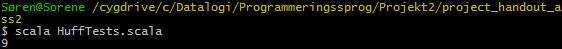
\includegraphics{test1.png}
As can be seen, the weight of the input tree is specified to 9, which is correctly returned. 

\subsection{def combine(left: HuffTree, right: HuffTree): HuffTree}
We once again "hardcode" our trees since we do not have the functionality to construct them otherwise until later. 
\lstinputlisting{test2.scala}
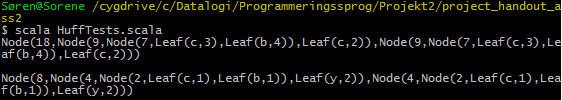
\includegraphics{test2.png}
The trees are simply added as subtrees to a new node, as can be seen. The new weight is calculated correctly. 


\subsection{def frequencies(chars: List[Char]): List[(Char, Int)]}
We input a list of characters as follows:
\lstinputlisting{tesst3.scala}
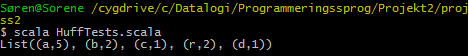
\includegraphics{test3.png}
We get a list of tuples of char and int as desired, and we see that the int corresponds to the number of occurences in our string of chars. 

\subsection{def combineTrees(trees: SortedSet[HuffTree])}
We still don't have a way to create CodeTrees (we're almos there!) so we use tree1 and tree2 from our previous test, for this test, as follows:
\lstinputlisting{test4.scala}
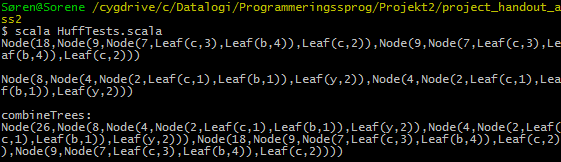
\includegraphics{test4.png}
We get the correct result.
The input list only has two elements, which is not that much, but it is still enough to see that we utilize both cases. We will see in later tests by extension that this method works for SortedSet with more than 2 elements. 
\subsection{def createCodeTree(chars: List[Char]): HuffTree}
We create 3 different lists. The last one has only a single element, to test this case as well. 
\lstinputlisting{test5.scala}
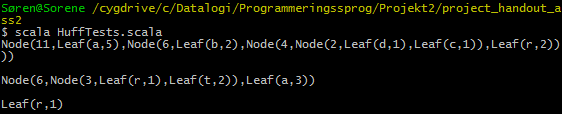
\includegraphics{test5.png}
We see that the Huffman Trees correspond to the input strings. The Most often used letters gets the shortest encodings as wished, and the rarely used letters get the longer encodings. In the case of just a single element, we get just a leaf, with that element. It actually ought to be Node(1,Leaf(r,1),Nil).
So our implementaiton actually does not work for just the case of just one single character. Arguably this is okay, since such cases are not interesting from a Huffman encodings perspective. But, optimally our implementation ought to produce the correct output in this case, which it doesn't. By extension we see that \textbf{combineTrees} works on SortedSet with more than 2 elements, due to our implementation. 

\subsection{def convert(tree: HuffTree): CodeTable}
We create a code tree, and feed it to convert. The result can be seen below.
\lstinputlisting{test6.scala}
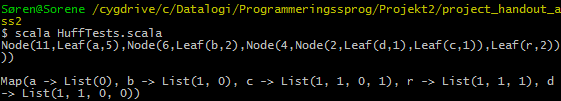
\includegraphics{test6.png}
The notation can be hard to read, but the reader can verify that the mappings obtained are correct. Initial tests revealed the need for a \textbf{reverse} in our implementation, and as can be seen it works. 


\subsection{def codeBits(table: CodeTable)(char: Char): List[Bit]}
We try obtaining the bits for the encoding of 'r' and 'd' using the codetable from the previos test.
\lstinputlisting{test7.scala}
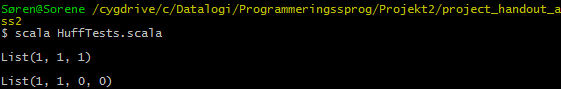
\includegraphics{test7.png}
If we compare this to the result from the test of \textbf{convert} we see that we obtain the correct results. 

\subsection{encode(table:CodeTable)(text: List[Char]): List[Bit]}
We once again use the string "abracadabra", create a codetree using it, and then test encode, on the same string. "abracadabra". 
\lstinputlisting{test8.scala}
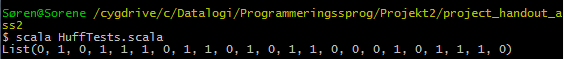
\includegraphics{test8.png}
Comparing the result to the Mapping obtained in the test of \textbf{convert}, we see that the result here is correct as well. 


\subsection{getLetter(tree: HuffTree, bits: List[Bit]): (Char, List[Bit])}
Here we compare the result of \textbf{encode} with the result of \textbf{getLetter}, on the same string as before.  
\lstinputlisting{test9.scala}
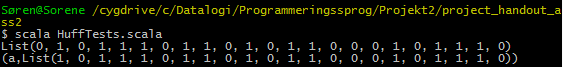
\includegraphics{test9.png}
As can be seen, the result is a tuple, with the first character we obtain, namely the 'a', as well as the remaining list, which can be seen to correspond to the previous result, with the leading 0 now decoded into the letter a. By extension, this function will be tested further in our last test of..

\subsection{def decode(tree: HuffTree)(bits: List[Bit]): List[Char]}
We create a codetree, encode the string from which it was made, print the codetable for readability, and then decode the list of bits that we encoded, to see wether the result is the same, using the supplied \textbf{edTest}
\lstinputlisting{test10.scala}
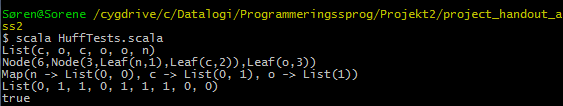
\includegraphics{test10.png}
We obtain a tree that corresponds to a HuffTree of the supplied list. We get the correct mapping of characters to their respective bit encodings. We get the correct encoding of the string that was used to create the codeTable. The test wether encoding and decoding of the string is the same, using \textbf{edTest} yields true. It seems as though everything has come together, and works. 
\newline
\\
As we saw in the test of createCodeTree, our implemetation does not consider (and work for) the case where a list is made up of the same character only. Consider the following test: 
\lstinputlisting{test11.scala}
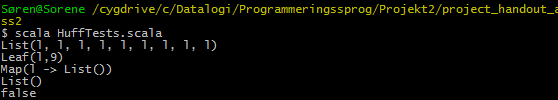
\includegraphics{test11.png}
Due to the implementation of \textbf{combineTrees},  and by entension \textbf{createCodeTree} and \textbf{convert}, a single element in the inputstring results in, as can be seen Leaf(l,9). The correct answer would be Node(9,Leaf(l,9),Nil). Our implementation does not consider this - it is an easy fix however. One could insert standard characters to ensure that it would always work, or test for this specific case. This was not done, however, due to the fact that a Huffman Encoding of just a single element is wildly uninterresting. It is not hard to make the most efficient encoding of just a single element. 
\newline
\\
We have a similar result if our string is just the empty string. Testing with this, results in a NoSuchElement.Exception, since we eventually end up with an empty map. 
\newline
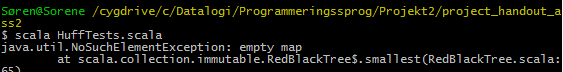
\includegraphics{testempty.png}
\subsection{Test for clarity}
Here we've chosen the input of "abbcccddddeeeee" to have an increasing frequency, so the resulting tree and encoding/decoding is easier to follow for the reader. 
\newline
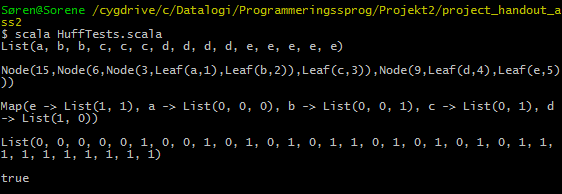
\includegraphics{test13.png}
Here one can see that the more frequent characters get the shorter encodings, and the less frequent get the longer encodings. No encoding is the prefix of another.
\subsection{Test on alphabet}
We've seen tests on simple words having chars with somewhat high frequencies. We should test the opposite! What better input that a string consisting of the entire alphabet "abcdefghijklmnopqrstuvxzy" (disclamer: this might not be the correct listing of the alphabet). The HuffTests.scala is the same as in the test of decode, just with our new string. The result is as follows:
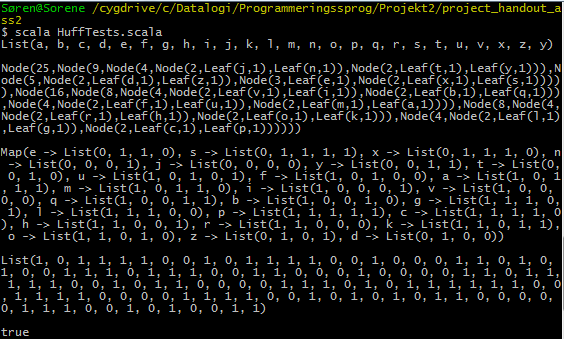
\includegraphics{test12.png}
All characters have a unique encoding, where none is a prefix of another, as desired.
\section{Conclusion}
Using pattern matching, recursion, as well as mapping we have succesfully implemented Huffman encoding with a functional approach. We have seen through our tests that the implementation is succesfull (on meaningfull input), and in the implementation section it can be seen that the approach is a functional one. The test cases chosen where meant to portray cases of interest i.e. having them differ in some way related to Huffman Encoding.  
\newline
\\
One of the last test concluded that on input of the empty string, or a string with only the same elements repeated a number of times, our implementation does not work. Good code terminates on every input and gives the correct answer, so this is unfortunate. 
\newline
 We argue that since the result of these case are of no use in the first place, no reason was seen to account for these cases. A fix would be to explicitly test for these cases, and print some sort of error message to warn the user. But if you want to use the functionality of this implementation, or Huffman encoding just generally, the cases of just a single element or no elements at all in the inputstring are irrelevant. When implementing methods, you should account for all possible input, but the user also holds the responsibility of not inputting nonsense. 
\section{Appendix- Huffman.scala}
\lstinputlisting{Huffman.scala}

\end{document}